\documentclass[]{swapnanil-resume}
\usepackage{fancyhdr}
\usepackage{graphicx}
\usepackage{tikz}
\usepackage{eso-pic}
\pagestyle{fancy}
\fancyhf{}


\begin{document}
\AddToShipoutPictureBG*{%
    \begin{tikzpicture}[remember picture, overlay]
        \node[anchor=north east, inner sep=0] at (current page.north east) {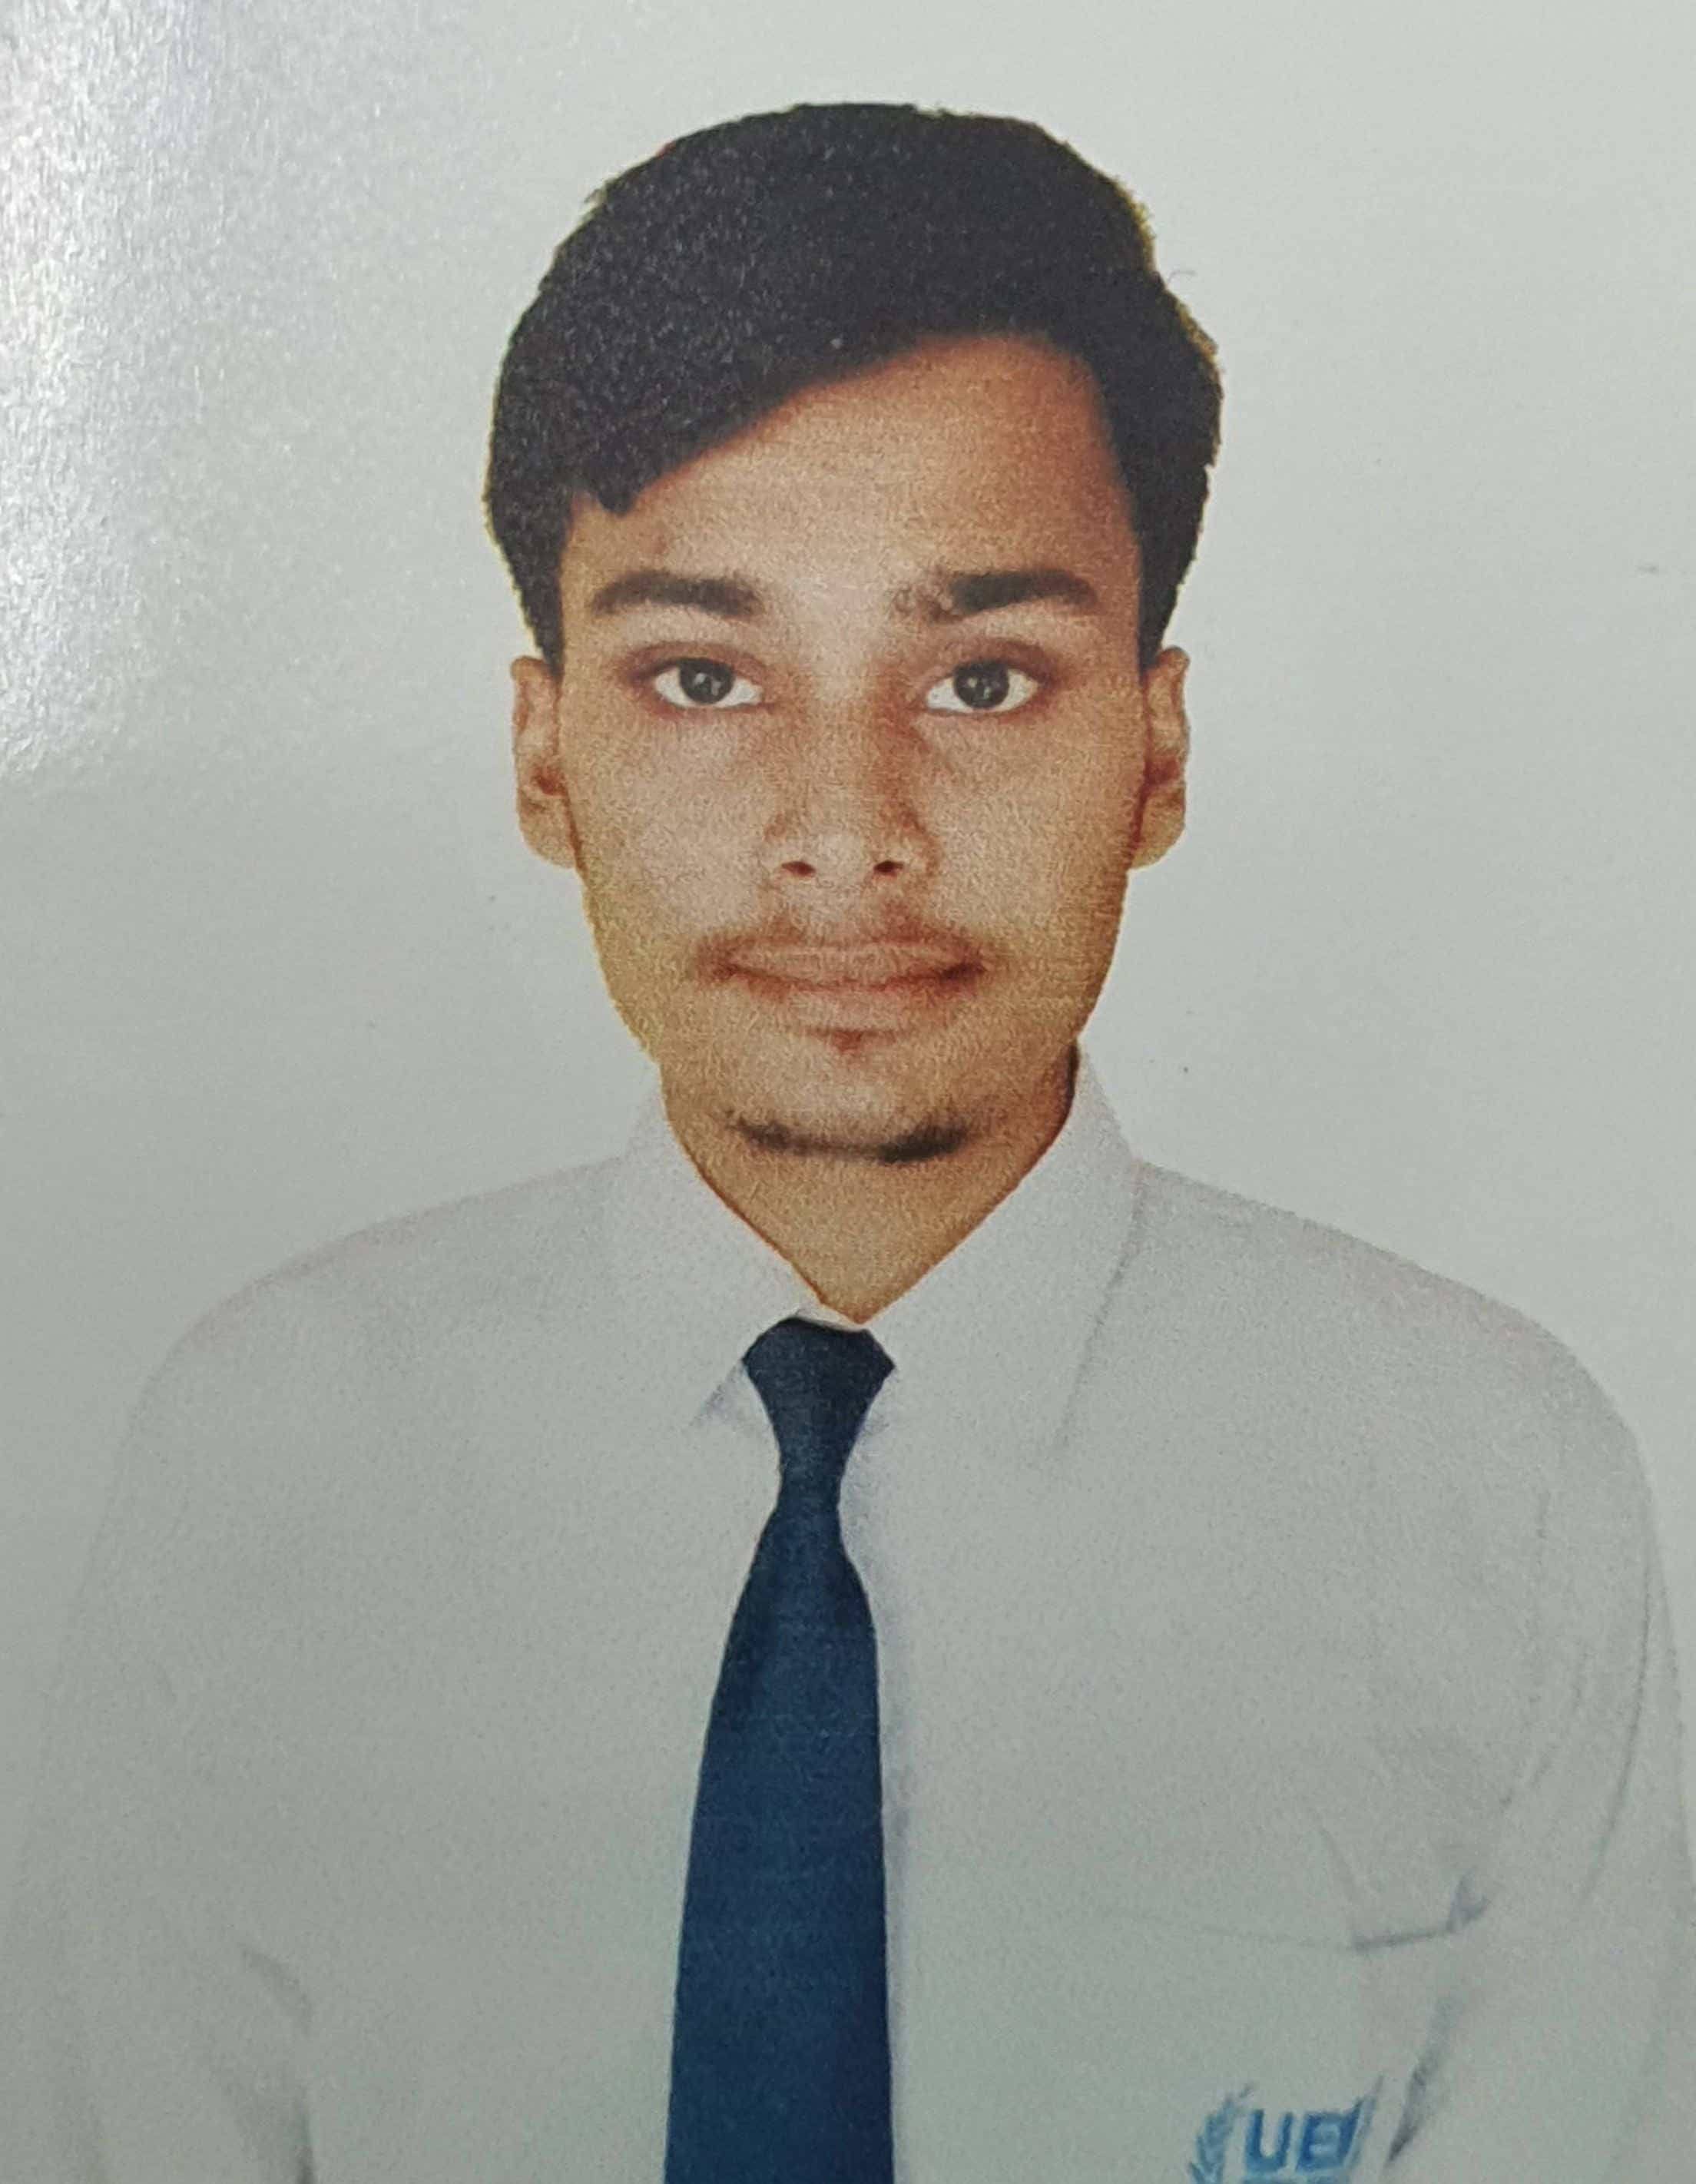
\includegraphics[width=2.3cm]{mypic.jpg}};
    \end{tikzpicture}%
}
%%%%%%%%%%%%%%%%%%%%%%%%%%%%%%%%%%%%%%
%
%     LAST UPDATED DATE
%
%%%%%%%%%%%%%%%%%%%%%%%%%%%%%%%%%%%%%%
%\lastupdated

%%%%%%%%%%%%%%%%%%%%%%%%%%%%%%%%%%%%%%
%
%     TITLE NAME
%
%%%%%%%%%%%%%%%%%%%%%%%%%%%%%%%%%%%%%%

\namesection{Swapnanil}{Chakraborty}{ \urlstyle{same}
\href{mailto:swapnanil2@proton.me}{swapnanil2@proton.me} | +917679015958 | Kolkata
}

%%%%%%%%%%%%%%%%%%%%%%%%%%%%%%%%%%%%%%
%
%     COLUMN ONE
%
%%%%%%%%%%%%%%%%%%%%%%%%%%%%%%%%%%%%%%

\begin{minipage}[t]{0.33\textwidth} 

%%%%%%%%%%%%%%%%%%%%%%%%%%%%%%%%%%%%%%
%     EDUCATION
%%%%%%%%%%%%%%%%%%%%%%%%%%%%%%%%%%%%%%

\section{Education} 

\subsection{University of Engineering and Management}
\descript{B.Tech in Computer Science}
\location{May 2020 | Kolkata, WB}
CGPA(Upto 7th semester): 8.35/10

\sectionsep

\subsection{Burdwan Model
School}
\descript{C.B.S.E (Class XII)}
\descript{Percentage: 61.6\%}
\descript{2020}

\sectionsep

\subsection{St. Joseph's School}
\descript{I.C.S.E (Class X)}
\descript{Percentage: 78.5\%}
\descript{2018}

\sectionsep

%%%%%%%%%%%%%%%%%%%%%%%%%%%%%%%%%%%%%%
%     LINKS
%%%%%%%%%%%%%%%%%%%%%%%%%%%%%%%%%%%%%%

\section{Links} 
Github:// \href{https://github.com/swapnanil1}{\bf swapnanil1} \\
LinkedIn://  \href{https://www.linkedin.com/in/swapnanil-chakraborty-046887294/}{\bf swapnanil} \\
YouTube://  \href{https://www.youtube.com/@TalkingTechTeam}{\bf TalkingTech} \\
Twitter://  \href{https://twitter.com/swapnanil111}{\bf @swapnanil} \\

\sectionsep
%%%%%%%%%%%%%%%%%%%%%%%%%%%%%%%%%%%%%%
%     COURSEWORK
%%%%%%%%%%%%%%%%%%%%%%%%%%%%%%%%%%%%%%

\section{Coursework}
\subsection{Undergraduate}
Data Structure \& Algorithms \\
Design \& Analysis of Algorithms \\
Object Oriented Programming \\
Database Management System \\
Operating System \\
Computer Networks \\
Linux \& CLI
\sectionsep

%%%%%%%%%%%%%%%%%%%%%%%%%%%%%%%%%%%%%%
%     SKILLS
%%%%%%%%%%%%%%%%%%%%%%%%%%%%%%%%%%%%%%

\section{Skills}
\subsection{Programming}
\descript{Experienced:}
Java \textbullet{} C++ \textbullet{} MySQL 
\\
\descript{Familiar:}
HTML \textbullet{} CSS \textbullet{} Javascript \\

%%%%%%%%%%%%%%%%%%%%%%%%%%%%%%%%%%%%%%
%
%     COLUMN TWO
%
%%%%%%%%%%%%%%%%%%%%%%%%%%%%%%%%%%%%%%
\end{minipage} 
\hfill
\begin{minipage}[t]{0.66\textwidth} 

%%%%%%%%%%%%%%%%%%%%%%%%%%%%%%%%%%%%%%
%     EXPERIENCE
%%%%%%%%%%%%%%%%%%%%%%%%%%%%%%%%%%%%%%

\section{Projects}
\runsubsection{KaiOS Application}
\descript{| Implemented Hotspot on JioPhones  }
\location{October 2023 | Personal Project }
\vspace{\topsep}
\begin{tightemize}
\item Developed KaiOS Jailbreaking Guide, emphasizing JavaScript, Linux, and KaiOS app packaging.
\item Created Hotspot App for KaiOS without native support, showcasing technical proficiency.
\item Detailed step-by-step instructions for official and advanced jailbreaking methods.
\item Implemented firmware downgrading, image modification, and post-installation steps for device security.
\end{tightemize}
\sectionsep
    
\runsubsection{Web App}
\descript{| A Dynamic News Portal Web Based 
Application }
\location{March 2023 | UEM,Kolkata}
\begin{tightemize}
\item Designed and developed a dynamic news portal web application using HTML, CSS, and JS.
\item Created an intuitive user interface with responsive design.
\item Demonstrated proficiency in  frontend design and backend scripting.
\end{tightemize}
\sectionsep

\runsubsection{App Development}
\descript{| Android + Personal 
Finance App }
\location{Feb 2022 | UEM,Kolkata}
\begin{tightemize}
\item Developed a user-friendly Android app using Java to manage personal finances.
\item Implemented budget tracking and expense management features.
\item Included expense categories for better financial organization.
\item Created a user interface for easy input of expenses and display of remaining budget.
\end{tightemize}
\sectionsep

\runsubsection{Game Development}
\descript{| Unreal Engine }
\location{October 2021 | UEM,Kolkata }
\begin{tightemize}
\item Create an FPS game set in a noir-style city environment
\item Design a player character with shooting controls.
\item Add enemy bot generation with hunting behavior.
\item Design a simple UI to display player score.
\end{tightemize}
\sectionsep
%%%%%%%%%%%%%%%%%%%%%%%%%%%%%%%%%%%%%%
%     Certifications
%%%%%%%%%%%%%%%%%%%%%%%%%%%%%%%%%%%%%%

\section{Certifications}
\runsubsection{Python Crash Course}
\descript{| Coursera}
\location{March 19, 2023 }
I have successfully acquired a fundamental understanding of Python, encompassing its core concepts and syntax. You can view my certificate of completion for this course \textbf{\href{https://coursera.org/share/b71698928aaa068338abf1bd936cc1b3}{Coursera}} .

\runsubsection{AWS Cloud Essentials}
\descript{| Coursera}
\location{Apr 30, 2023}
The 'AWS Cloud Technical Essentials' course on Coursera has provided me with foundational knowledge of Amazon Web Services (AWS) and its global infrastructure.. You can view my certificate of completion for this course \textbf{\href{https://coursera.org/share/5fca237b7c7400c97aad8745162c9c29}{Coursera}} .
\sectionsep
%%%%%%%%%%%%%%%%%%%%%%%%%%%%%%%%%%%%%%
%     AWARDS
%%%%%%%%%%%%%%%%%%%%%%%%%%%%%%%%%%%%%%

\section{Achievements} 
\begin{tabular}{rll}
2020	     & 3\textsuperscript{rd} & Debate Competition held at Kashiram Das Institution\\
2021     & 3\textsuperscript{rd} & at District level in Long Jump  \\
2022	     & 13th  & Place in the UEM, Coding Competition\\
2022     & 103\textsuperscript{th} & in Cycling Competition held by UEM/IEM \\
\end{tabular}
\sectionsep

\end{minipage} 
\end{document}  \documentclass[]{article}

